\everymath{\displaystyle}
\documentclass{beamer}
% \documentclass[handout]{beamer}

%\usepackage[pdftex]{color,graphicx}
\usepackage{amsmath,amssymb,amsfonts}

\mode<presentation>
{
  % \usetheme{Darmstadt}
  % \usetheme[hideothersubsections]{Hannover}
  % \usetheme[hideothersubsections]{Goettingen}
  \usetheme[hideothersubsections, right]{Berkeley}

  \usecolortheme{seahorse}
  % \usecolortheme{dolphin}
  \usecolortheme{rose}
  % \usecolortheme{orchid}

  \useinnertheme[shadow]{rounded}

  \setbeamercovered{transparent}
  % or whatever (possibly just delete it)
}

\mode<handout>{
  \setbeamercolor{background canvas}{bg=black!5}
  \usepackage{pgfpages}
  \pgfpagesuselayout{4 on 1}[a4paper,border shrink=5mm, landscape]
}

\usepackage[brazilian]{babel}
% or whatever

% \usepackage[latin1]{inputenc}
\usepackage[utf8]{inputenc}
% or whatever

\usepackage{times}
%\usepackage[T1]{fontenc}
% Or whatever. Note that the encoding and the font should match. If T1
% does not look nice, try deleting the line with the fontenc.


\title%[] % (optional, use only with long paper titles)
{Comparando médias de 2 grupos}

\subtitle
{Intervalos de Confiança da diferença entre as médias} % (optional)

\author%[] % (optional, use only with lots of authors)
{Felipe Figueiredo}% \and S.~Another\inst{2}}
% - Use the \inst{?} command only if the authors have different
%   affiliation.

\institute[] % (optional, but mostly needed)
{
}
  % \inst{1}%
  % Department of Computer Science\\
  % University of Somewhere
  % \and
  % \inst{2}%
  % Department of Theoretical Philosophy\\
  % University of Elsewhere}
% - Use the \inst command only if there are several affiliations.
% - Keep it simple, no one is interested in your street address.

\date%[] % (optional)
{}

% \subject{Talks}
% This is only inserted into the PDF information catalog. Can be left
% out. 



% If you have a file called "university-logo-filename.xxx", where xxx
% is a graphic format that can be processed by latex or pdflatex,
% resp., then you can add a logo as follows:

\pgfdeclareimage[height=1.6cm]{university-logo}{../logo}
\logo{\pgfuseimage{university-logo}}



% Delete this, if you do not want the table of contents to pop up at
% the beginning of each subsection:
\AtBeginSubsection[]
%\AtBeginSection[]
{
  \begin{frame}<beamer>{Sumário}
    \tableofcontents[currentsection,currentsubsection]
  \end{frame}
}


% If you wish to uncover everything in a step-wise fashion, uncomment
% the following command: 

% \beamerdefaultoverlayspecification{<+->}


\begin{document}

\begin{frame}
  \titlepage
\end{frame}

\begin{frame}{Sumário}
  \tableofcontents
  % You might wish to add the option [pausesections]
\end{frame}


%% Template
% \section{}

% \subsection{}

% \begin{frame}{}
%   \begin{itemize}
%   \item 
%   \end{itemize}
% \end{frame}

% \begin{frame}
%   \begin{columns}
%     \begin{column}{5cm}
%     \end{column}
%     \begin{column}{5cm}
%     \end{column}
%   \end{columns}
% \end{frame}

% \begin{frame}{}
%   \includegraphics[height=0.4\textheight]{file1}
%   \includegraphics[height=0.4\textheight]{file2}
%   \includegraphics[height=0.4\textheight]{file3}
%   \begin{figure}
%     \caption{}
%   \end{figure}
% \end{frame}

% \begin{frame}{}
%   \begin{definition}
%   \end{definition}
%   \begin{example}
%   \end{example}
%   \begin{block}{Exercício}
%   \end{block}
% \end{frame}

\section[t de Student]{A distribuição t de Student}

\subsection{A distribuição t de Student}

\begin{frame}{Recapitulando}
  \begin{itemize}
  \item Vimos que o IC é composto de 3 componentes
    \begin{itemize}
    \item a média $\bar{x}$ (tendência central)
    \item o erro padrão da média (SEM)
    \item um tal de $t^{*}$, que depende de $n$
    \end{itemize}
  \item Como N era grande, utilizamos $t^{*} \approx 2$
    \bigskip
  \item Mas de onde vem esse $t^{*}$? Qual seria o valor correto?
  \end{itemize}
\end{frame}

\begin{frame}{A distribuição T de Student}
  \begin{center}
    
\includegraphics[height=\textheight]{Cap5/Guinness}
  \end{center}
\end{frame}

\begin{frame}{A distribuição T de Student}
  \begin{center}
    
\includegraphics[height=\textheight]{Cap5/Student-Guinness}
  \end{center}
\end{frame}

\begin{frame}{A distribuição t de Student}
  \begin{itemize}
  \item Student (pseudônimo de W. S. Gossett [1876-1937], trabalhando
    para a cervejaria Guiness) criou uma distribuição que melhor se
    aproxima dos dados de amostras pequenas
%  \item É semelhante à Normal padrão, mas tem variância maior
  \item Tem um parâmetro \alert{graus de liberdade} ({\em df} em inglês) vinculado ao tamanho da amostra $n$.
    % \begin{displaymath}
    %   gl = n-1
    % \end{displaymath}
  \end{itemize}
\end{frame}

\begin{frame}{A distribuição t de Student}
  \begin{figure}
    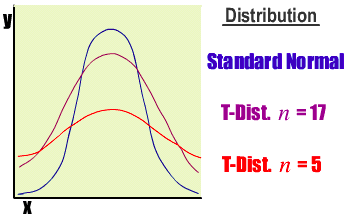
\includegraphics[height=0.7\textheight]{Inf_II/t_graph}
    \caption{A distribuição t de Student}
  \end{figure}
\end{frame}

\begin{frame}{Propriedades da distribuição t}
  \begin{itemize}
  \item A distribuição tem forma de sino (simétrica, assim como a
    distribuição Normal)
  \item Reflete a maior variabilidade inerente às amostras pequenas
  \item O formato da curva depende do tamanho da amostra $n$
  \item Quanto mais graus de liberdade (df $\approx$ dados), mais a distribuição
    $t$ se parece com a distribuição Normal
  \end{itemize}
\end{frame}

% \begin{frame}{A tabela t}
%   \begin{center}
%     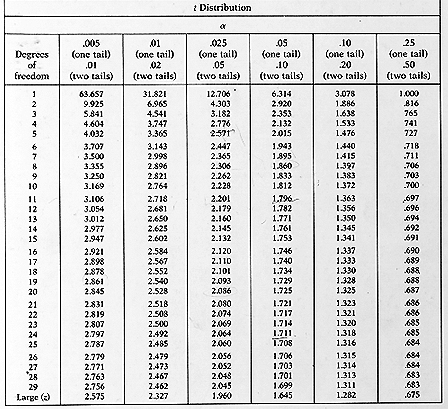
\includegraphics[height=0.9\textheight]{Inf_II/t_table}
%   \end{center}
% \end{frame}


\begin{frame}{IC da média (aula passada)}
  \begin{exampleblock}{ICs dos exemplos}
    \begin{itemize}
    \item IC do ex. 5.1 (PS de 100 alunos): [120.6, 126.2] mmHg
    \item IC do ex. 5.2 (PS de   5 alunos): [79.2, 118.8] mmHg
    \end{itemize}
  \end{exampleblock}
  \begin{block}{Pense...}
    Observe os tamanhos dos ICs.
  \end{block}
\end{frame}

\begin{frame}{Alguns valores de t, para diferentes graus de liberdade}
  \begin{itemize}
  \item $N = 5\ (df = 4) \Rightarrow t = 2.776$
  \item $N = 10\ (df = 9) \Rightarrow t = 2.262$
  \item $N = 15\ (df = 14) \Rightarrow t = 2.145$
  \item $N = 20\ (df = 19) \Rightarrow t = 2.093$
  \item $N = 30\ (df = 29) \Rightarrow t = 2.045$
  \end{itemize}
  \begin{block}{Pense...}
    Qual é a relação entre N e o tamanho do IC?

    % \begin{displaymath}
    %   IC: \bar{x} \pm t^{*} \times SEM
    % \end{displaymath}
    \begin{displaymath}
      \left[ \bar{x} - t^{*} SEM,\ \ \bar{x} + t^{*} SEM \right]
    \end{displaymath}
  \end{block}
\end{frame}

\begin{frame}{Alguns valores de t, para diferentes graus de liberdade}
  \begin{itemize}
  \item $N = 5\ (df = 4) \Rightarrow t = 2.776$
  \item $N = 10\ (df = 9) \Rightarrow t = 2.262$
  \item $N = 15\ (df = 14) \Rightarrow t = 2.145$
  \item $N = 20\ (df = 19) \Rightarrow t = 2.093$
  \item $N = 30\ (df = 29) \Rightarrow t = 2.045$
  \end{itemize}
  \begin{block}{Observe que...}
    \begin{itemize}
    \item $df = N - 1$
    \item Para N  grande, $t \rightarrow 1.960$
    \end{itemize}
    Por isso usamos o valor aproximado $2$ no primeiro exemplo.
  \end{block}
\end{frame}

\begin{frame}[label=exercicio5.4]{Exercício 4 (cap 5)}
  \begin{exampleblock}{Exercício 4 do cap 5}
    Os níveis de soro (fator Y) foram medidos em 100 mulheres não-grávidas, e 100 mulheres com até 3 meses de gravidez. Os ICs dos valores dos soros em ambos os grupos são:
    \begin{itemize}
    \item Não-grávidas: [90.0, 96.0]
    \item Grávidas: [105.4, 114.6]
    \end{itemize}

    \bigskip
    {\bf O fator Y médio é diferente em mulheres grávidas e não-grávidas?}
  \end{exampleblock}
\end{frame}

\begin{frame}{Pense}
  \begin{exampleblock}{}
    \begin{itemize}
    \item Não-grávidas: [90.0, 96.0]
    \item Grávidas: [105.4, 114.6]
    \end{itemize}
  \end{exampleblock}
  \begin{itemize}
  \item o SEM informa quão bem você conhece a média de cada grupo
  \item Os ICs não tem sobreposição $\Rightarrow$ 2 populações diferentes
  \item Como comparar estes dois grupos?
  \end{itemize}
\end{frame}

\section[IC diferença 2 médias]{Intervalo de Confiança da diferença entre duas médias}

\subsection{Interpretação}

\begin{frame}{Diferença entre 2 médias}
  \begin{itemize}
  \item Frequentemente precisamos dividir os dados em dois grupos e
    comparar as médias.
  \item Isto pode ser usado para se estudar o efeito de um tratamento
    em relação a um grupo controle
  \item ou mesmo para se comparar dois tratamentos diferentes.
  \end{itemize}
\end{frame}

\begin{frame}{Diferença entre 2 médias}
  \begin{itemize}
  \item Para comparar duas médias $\bar{x_1}$ e $\bar{x_2}$, consideramos a diferença $\bar{x_1} - \bar{x_2}$
  \item Raciocínio: se as médias forem aproximadamente iguais, a
    diferença será aproximadamente zero
  \item Além disso, se $\bar{x_1}$ for maior que $\bar{x_2}$, a diferença será positiva
  \item Analogamente, se $\bar{x_1}$ for menor que $\bar{x_2}$, a diferença será negativa
  \end{itemize}
\end{frame}

\begin{frame}{Erro padrão da diferença}
  \begin{itemize}
  \item Lembre-se que para cada grupo: $SEM = \frac{DP}{\sqrt{N}}$
  \item Para a diferença entre 2 grupos, ``somamos'' os SEM
  \item Mas esta ``soma'' não é direta!
  \item É preciso levar em conta o uso do quadrado/raiz quadrada do DP (aula de variabilidade)
  \end{itemize}
  \begin{block}{}
      \begin{displaymath}
    SE = \sqrt{SEM_1^2 + SEM_2^2}
  \end{displaymath}
  \end{block}
\end{frame}

\begin{frame}{Premissas}
  \begin{itemize}
  \item As amostras foram selecionadas aleatoriamente das respectivas populaçoes
  \item As populações são Normais (Gaussianas)
  \item As duas populações possuem DP idênticos
  \item Todos os indivíduos de cada grupo vêm da mesma população
  \item Cada indivíduo é independente de todos os outros
  \end{itemize}
\end{frame}

\againframe{exercicio5.4}

\begin{frame}{Cálculo exercício 5.4/7.1}
  \begin{exampleblock}{Diferenças: Exercício 5.4 (e 7.1)}
    \begin{itemize}
    \item Média grávidas: $\bar{x_1} = 110$ unidades/ml
    \item Média não-grávidas: $\bar{x_2} = 93$ unidades/ml
    \item Diferença entre as médias: $\bar{x_d} = \alert{17}$ unidades/ml
    \item SEM da diferença: \alert{2.75} unidades/ml
    \item $N_1=100, N_2=100 \Rightarrow df = (100 -1) + 1(00 - 1) = \alert{198}$
    \item $t^{*} = \alert{1.97}$
    \end{itemize}
  \end{exampleblock}
  \begin{exampleblock}{IC}
    \centering
    [11.6, 22.4] unidades/ml
  \end{exampleblock}
  E o que significa isso?
\end{frame}

\begin{frame}{Solução}
    \begin{exampleblock}{IC}
    \centering
    [11.6, 22.4] unidades/ml
  \end{exampleblock}
  \begin{itemize}
  \item Estamos 95\% certos que a diferença real entre os grupos está entre 11.6 e 22.4
  \item Conclusão: o fator Y de uma mulher grávida entre 11.6 e 22.4 unidades/ml maior que em uma mulher não grávida
  \end{itemize}
\end{frame}

\subsection{Participantes: pareados ou não-pareados?}

\begin{frame}{Grupos não-pareados x pareados}
  Aula que vem...
\end{frame}

\begin{frame}{Grupos pareados}
  \begin{itemize}
  \item Até agora assumimos que os grupos e participantes são {\bf independentes}
  \item Existe um caso importante em que pode-se considerar que eles são dependentes: quando são pareados
  \item Isto significa que cada participante de um grupo tem um correspondente no outro
  % \item 
  \end{itemize}
\end{frame}

\begin{frame}{Comparação pareada}
  
\end{frame}

\end{document}
